\documentclass[compress]{beamer}

\usetheme{CambridgeUS}
\usecolortheme{rose}

\usepackage{amsmath,amsfonts,amssymb}
\usepackage{caption}
\captionsetup[table]{labelformat=empty}

\title{AON: Towards Arbitrarily-Oriented Text Recognition}
\author[Presentor: Shih-Ming Wang]{Zhanzhan Cheng, Yangliu Xu, Fan Bai, Yi Niu, \\ Shiliang Pu, Shuigeng Zhou}
\institute[]{Presented by Shih-Ming Wang \\ ComputerVision Lab, UCSC}
\date{10-24-2018}
\subject{Computer Science}
\graphicspath{{img/}}


\begin{document}

\begin{frame}
    \maketitle
    \hypertarget{titlePage}{}
\end{frame}

\section{Motivation}
\begin{frame}{Motivation}
    \begin{block}{OCR in Practice}
        \begin{itemize}
            \item Uneven lighting, blurring
            \item Perspective distortion 
            \item Orientation
            \item Most traditional OCR system deals with regular tightly-bounded, horizontal texts
        \end{itemize} 
    \end{block}  
    \begin{figure}
        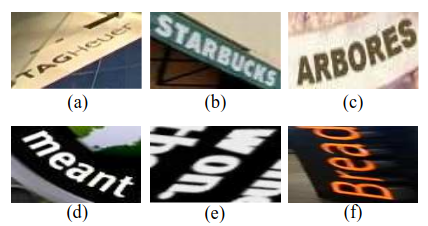
\includegraphics[height=.3\textheight]{motivation}
    \end{figure}
\end{frame}

\section{Previous Work}
\begin{frame}[allowframebreaks]{Previous Work}
    \begin{block}{Spatial Transformer Network Based Model}
        \begin{itemize}
            \item The model learns to rectify input image, rotation, etc.
            \item Hard to optimize transformation network without geometric groundtruth
            \item Requires tricks on initialisation of model weights to guarantee training convergence
        \end{itemize}
    \end{block}
    \begin{figure}
        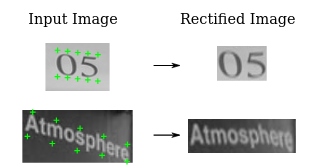
\includegraphics[height=.5\textheight]{rectify}
    \end{figure}
    \framebreak
    \begin{columns}
        \begin{column}[T]{.5\textwidth}
            \begin{block}{Attention Based Model}
                \begin{itemize}
                    \item Encode image into featuremap and use RNN to predict character sequences.
                    \item Does not work well when directly applied to irregular texts
                \end{itemize}

            \end{block}
        \end{column}
        \begin{column}[T]{.5\textwidth}
            \begin{figure}
                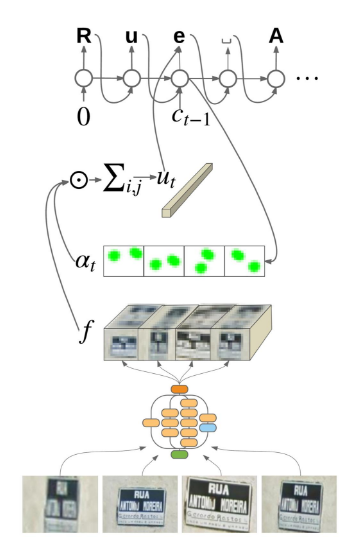
\includegraphics[width=.8\textwidth]{attention_model}
            \end{figure}
        \end{column}
    \end{columns}
\end{frame}

\section{Proposed Method}
\begin{frame}{Method Intuition}
    \begin{itemize}
        \item Extract feature of four direction and learn to weight them properly
    \end{itemize}
    \begin{figure}
        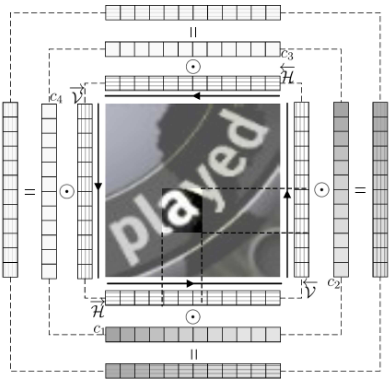
\includegraphics[width=.6\textheight]{method_intuition}
    \end{figure}
\end{frame}

\begin{frame}{Architecture Overview}
    \begin{columns}
        \begin{column}[T]{.5\textwidth}
            \begin{itemize}
                \item <1-> Basal CNN(BCNN): extract low level image features
                \item <2-> Arbitrary(AON): extract high level features in 4 direction and calculate character placement clue
                \item <3-> Filter Gate (FG): Combine the 4 features with the character placement clue
                \item <4-> Attention-based Decoder: predict character sequence from the combined features
            \end{itemize}
        \end{column}
        \begin{column}[T]{.5\textwidth}
            \begin{figure}
                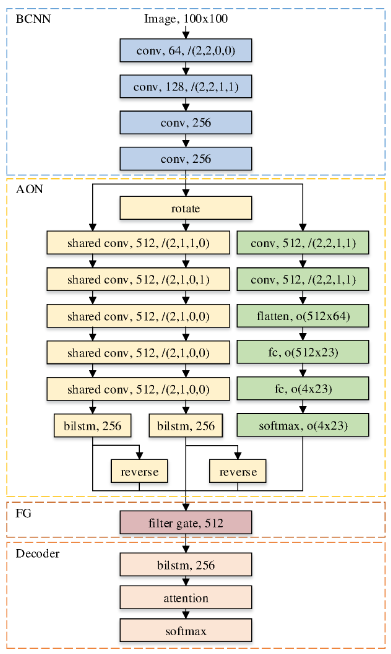
\includegraphics[width=\textwidth,height=.8\textheight]{arch}
            \end{figure}
        \end{column}
    \end{columns}
\end{frame}

\begin{frame}{Basal CNN}
    \begin{columns}
        \begin{column}[T]{.5\textwidth}
            \begin{itemize}
                \item Simple stacked CNN 
                \item The output must be square feature maps
            \end{itemize}
        \end{column}
        \begin{column}[T]{.5\textwidth}
            \begin{figure}
                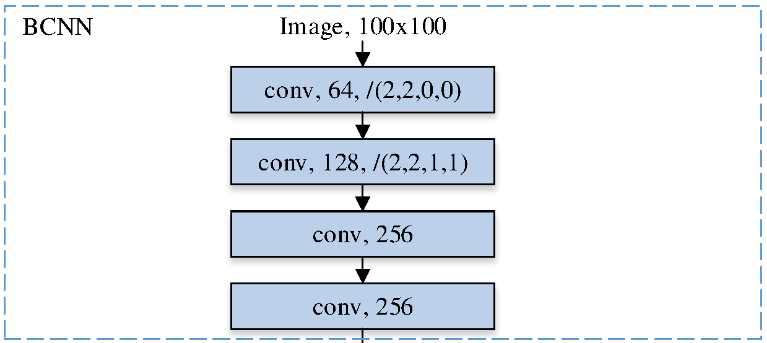
\includegraphics[width=\textwidth,height=.4\textheight]{bcnn}
            \end{figure}
        \end{column}
    \end{columns}
\end{frame}

\begin{frame}[allowframebreaks]{AON}
    \begin{columns}
        \begin{column}[T]{.5\textwidth}
            \begin{itemize}
                \item Consider ``left to right'': stacked CNN downsamples the input feature maps from original dimension $HxWxC$ to $1\times L \times D$
                \item Then feed the feature map to a bidirectional lstm to further encode the feature sequence (keeping the same dimension)
                \item ``right to left'' feature is just the reverse of ``left to right'' feature (which accelerates training convergence)
            \end{itemize}
        \end{column}
        \begin{column}[T]{.5\textwidth}
            \begin{figure}
                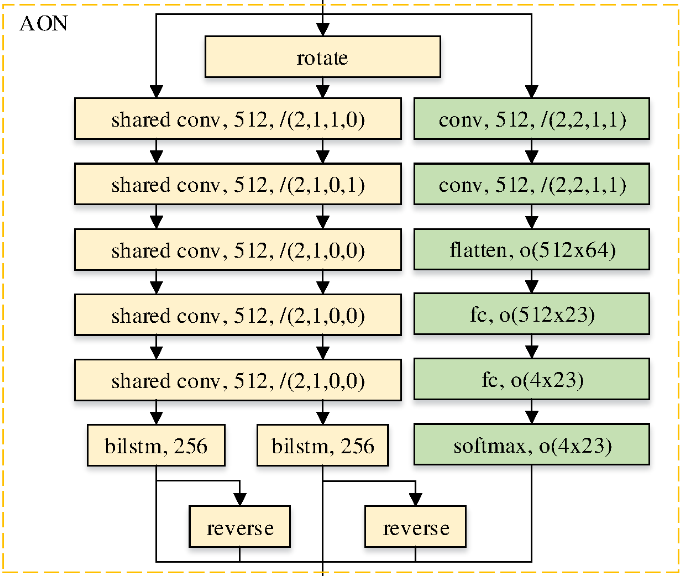
\includegraphics[width=\textwidth,height=.8\textheight]{aon}
            \end{figure}
        \end{column}
    \end{columns}
    \framebreak
    \begin{columns}
        \begin{column}[T]{.5\textwidth}
            \begin{itemize}
                \item For ``Up to down'', just rotate the input by 90 degree
                \item At the end we have 4 $L\times D$ feature maps
                \item In practice, horizontal and vertical CNN share parameters to avoid unbalanced orientation in the dataset
                \item The character placement clue network uses CNN-FC to calculate $4\times L$ weight
            \end{itemize}
        \end{column}
        \begin{column}[T]{.5\textwidth}
            \begin{figure}
                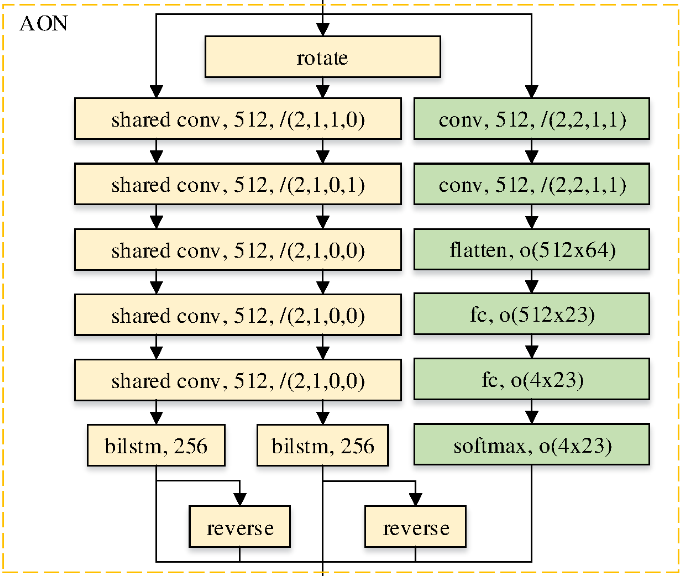
\includegraphics[width=\textwidth,height=.8\textheight]{aon}
            \end{figure}
        \end{column}
    \end{columns}
\end{frame}

\begin{frame}{Filter Gate}
    \begin{columns}
        \begin{column}[T]{.5\textwidth}
            \begin{itemize}
                \item Weighted sum of the 4 $L\times D$ features with the $4 \times L$ weights to get a $L \times D$ feature and then activate by $\tanh$ function
                \item For $i=1,\dots,L$
                    \begin{align*}
                        & \widehat{h_i}' = [\overrightarrow{\mathcal{H}_i}, \overleftarrow{\mathcal{H}_i}, \overrightarrow{\mathcal{V}_i}, \overleftarrow{\mathcal{V}_i}]c_i \\
                        & \widehat{h_i}'=\tanh(\widehat{h_i}') \\
                        & (\overrightarrow{\mathcal{H}_i}: D\times 1, c_i: 1\times 4)
                    \end{align*}
        \end{itemize}
        \end{column}
        \begin{column}[T]{.5\textwidth}
            \begin{figure}
                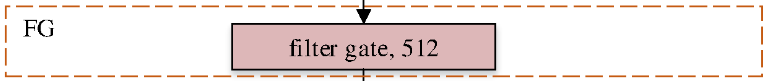
\includegraphics[width=\textwidth]{fg}
            \end{figure}
        \end{column}
    \end{columns}
\end{frame}

\begin{frame}{Attention Decoder}
    \begin{columns}
        \begin{column}[T]{.55\textwidth}
            \begin{itemize}
                \item Given previous output $y_{t-1}$, calculate the decoder input $g_t$, next state $s_t$ and next output $y_t$ as:
                    \begin{align*}
                        & g_t = \sum_{j=1}^L \alpha_{t,j} \widehat{h}_j \\
                        & s_t = RNN(y_{t-1},g_t,s_{t-1}) \\
                        & y_t = softmax(W^Ts_t)
                    \end{align*}
                \item $\alpha_t$ is a $1\times L$ vector and can be calculates in different ways. For e.g.
                    \begin{equation*}
                        \alpha_{t,j} = s_{t-1}^T M h_j
                    \end{equation*}
            \end{itemize}
        \end{column}
        \begin{column}[T]{.45\textwidth}
            \begin{figure}
                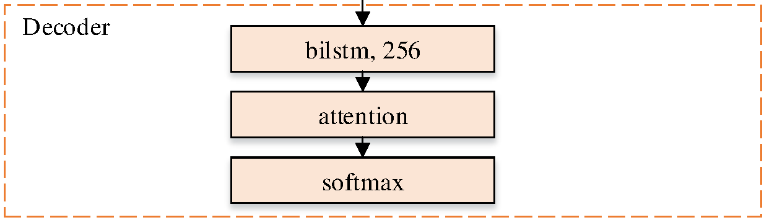
\includegraphics[width=\textwidth,height=.3\textheight]{decoder}
            \end{figure}
        \end{column}
    \end{columns}
\end{frame}

\section{Experiments}

\begin{frame}{Dataset}
    \begin{table}
        \centering
        \begin{tabular}{llll}
            Name            & Size  & Irregular & with lexicon \\ \hline\hline
            \
            SVT-Perspective & 639   & yes       & 50           \\ \hline
            CUTE80          & 288   & yes       & N/A          \\ \hline
            ICDAR 2015      & 2,077 & yes       & N/A          \\ \hline
            IIIT5K-Words    & 3,000 & no        & 50,1000      \\ \hline
            Street View     & 647   & no        & 50           \\ \hline
            ICDAR 2003      & 867   & no        & 50, Full     \\ \hline
        \end{tabular}
    \end{table}
    Trained on 12-million synthetic dataset.
\end{frame}


\begin{frame}[allowframebreaks]{Experiment Result}
    \begin{table}
        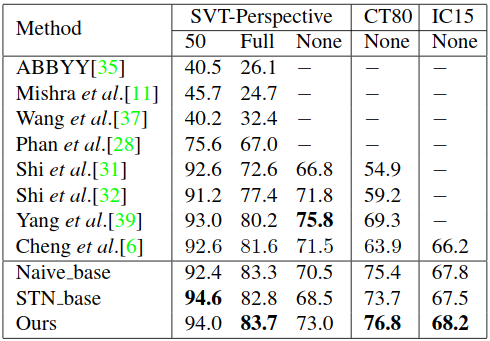
\includegraphics[height=.5\textheight]{pfirregular}
        \caption{Performance on irregular datasets.}
    \end{table}
    \begin{table}
        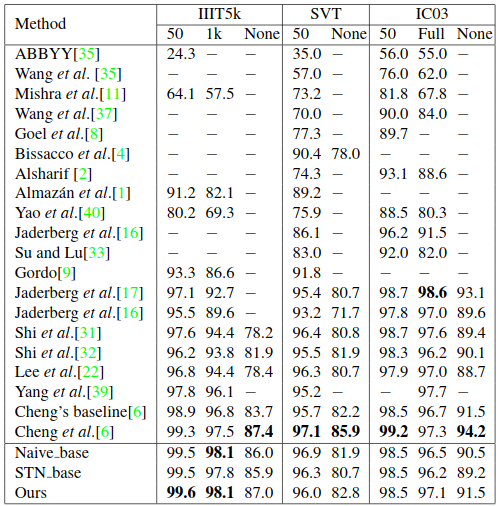
\includegraphics[height=.78\textheight]{pfregular}
        \caption{Performance on regular datasets.}
    \end{table}
\end{frame}

\section{AON Insight}
\begin{frame}{Generated Placement Clues}
    \begin{figure}
        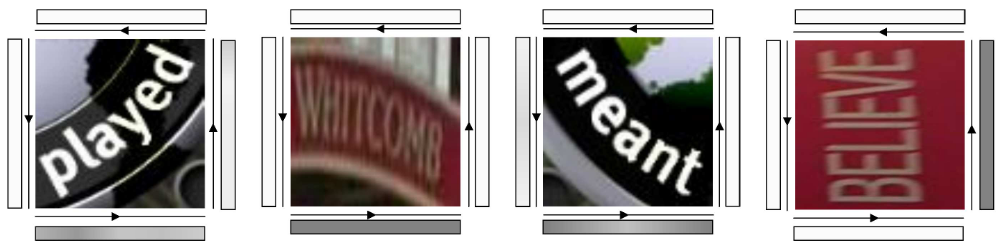
\includegraphics[width=\textwidth]{cnres}
    \end{figure}
\end{frame}

\begin{frame}{Text Placement Trends I}
    \begin{itemize}
        \item <+->Visualize the model proposed position for each character
        \item <+->At each time step we have character placement $\mathcal{C}$ ($4\times L$), attention mask $\alpha_t$ (4 $\times L$)
        \item <+->Geometrically, the image is divided into $L\times L$ patches, and we try to visualize at each time step, which patch are we looking at
        \item <+->position distribution
            \begin{equation*}
                dis = (d_1,d_2,d_3,d_4) = \mathcal{C} \odot \alpha_t \in \mathbb{R}^{4\times L}
            \end{equation*}
        \item <+->$d_{1j}$ measures the importance of the j's column in ``left-to-right'' feature and $d_{2j}$ measures that of ``right-to-left'' feature
        \item <+->Horizontal position at time step $t$
            \begin{equation*}
                x = \sum_{i=1}^2\sum_{j=1}^L j \times norm(d_{ij})
            \end{equation*}
    \end{itemize}
\end{frame}

\begin{frame}{Text Placement Trends II}
    \begin{figure}
        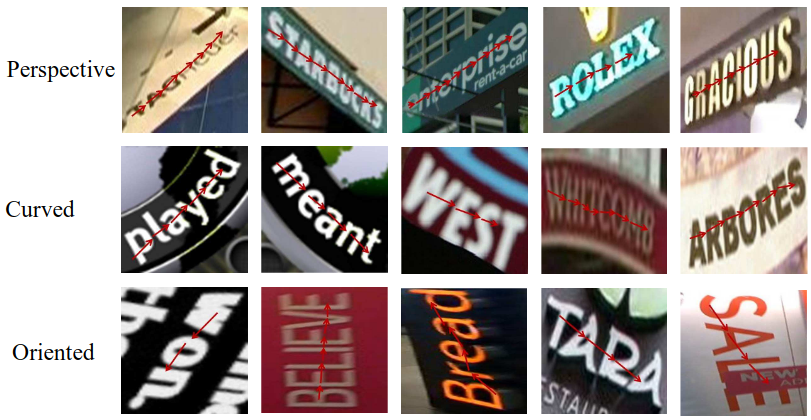
\includegraphics[width=\textwidth]{trends}
    \end{figure}
\end{frame}

\end{document}
